%%% Fiktivní kapitola s ukázkami tabulek, obrázků a kódu


%!TEX root = ../prace.tex

\chapter{Programátorská dokumentace}

Používání tabulek a grafů v~odborném textu má některá společná
pravidla a~některá specifická. Tabulky a grafy neuvádíme přímo do
textu, ale umístíme je buď na samostatné stránky nebo na vyhrazené
místo v~horní nebo dolní části běžných stránek. \LaTeX\ se o~umístění
plovoucích grafů a tabulek postará automaticky.

Každý graf a tabulku
očíslujeme a umístíme pod ně legendu. Legenda má popisovat obsah grafu
či tabulky tak podrobně, aby jim čtenář rozuměl bez důkladného
studování textu práce.

Na každou tabulku a graf musí být v~textu odkaz
pomocí jejich čísla. Na příslušném místě textu pak shrneme ty
nejdůležitější závěry, které lze z~tabulky či grafu učinit. Text by
měl být čitelný a srozumitelný i~bez prohlížení tabulek a grafů a
tabulky a grafy by měly být srozumitelné i~bez podrobné četby textu.

Na tabulky a grafy odkazujeme pokud možno nepřímo v~průběhu běžného
toku textu; místo \emph{\uv{Tabulka~\ref{tab03:Nejaka} ukazuje, že
    muži jsou v~průměru o~$9,9\,\rm kg$ těžší než ženy}} raději napíšeme
\emph{\uv{Muži jsou o~$9,9\,\rm kg$ těžší než ženy (viz
    Tabulka~\ref{tab03:Nejaka})}}.

\section{Tabulky}

\begin{table}[b!]

\centering
%%% Tabulka používá následující balíčky:
%%%   - booktabs (\toprule, \midrule, \bottomrule)
%%%   - dcolumn (typ sloupce D: vycentrovaná čísla zarovnaná na
%%%     desetinnou čárku
%%%     Všimněte si, že ve zdrojovém kódu jsou desetinné tečky, ale
%%%     tisknou se čárky.
%%% Dále používáme příkazy \pulrad a \mc definované v makra.tex

\begin{tabular}{l@{\hspace{1.5cm}}D{.}{,}{3.2}D{.}{,}{1.2}D{.}{,}{2.3}}
\toprule
 & \mc{} & \mc{\textbf{Směrod.}} & \mc{} \\
\pulrad{\textbf{Efekt}} & \mc{\pulrad{\textbf{Odhad}}} & \mc{\textbf{chyba}$^a$} &
\mc{\pulrad{\textbf{P-hodnota}}} \\
\midrule
Abs. člen     & -10.01 & 1.01 & \mc{---} \\
Pohlaví (muž) & 9.89   & 5.98 & 0.098 \\
Výška (cm)    & 0.78   & 0.12 & <0.001 \\
\bottomrule
\multicolumn{4}{l}{\footnotesize \textit{Pozn:}
$^a$ Směrodatná chyba odhadu metodou Monte Carlo.}
\end{tabular}

\caption{Maximálně věrohodné odhady v~modelu M.}\label{tab03:Nejaka}

\end{table}

U~\textbf{tabulek} se doporučuje dodržovat následující pravidla:

\begin{itemize} %% nebo compactitem z balíku paralist
\item Vyhýbat se svislým linkám. Silnějšími vodorovnými linkami
  oddělit tabulku od okolního textu včetně legendy, slabšími
  vodorovnými linkami oddělovat záhlaví sloupců od těla tabulky a
  jednotlivé části tabulky mezi sebou. V~\LaTeX u tuto podobu tabulek
  implementuje balík \texttt{booktabs}. Chceme-li výrazněji oddělit
  některé sloupce od jiných, vložíme mezi ně větší mezeru.
\item Neměnit typ, formát a význam obsahu políček v~tomtéž sloupci
  (není dobré do téhož sloupce zapisovat tu průměr, onde procenta).
\item Neopakovat tentýž obsah políček mnohokrát za sebou. Máme-li
  sloupec \textit{Rozptyl}, který v~prvních deseti řádcích obsahuje
  hodnotu $0,5$ a v~druhých deseti řádcích hodnotu $1,5$, pak tento
  sloupec raději zrušíme a vyřešíme to jinak. Například můžeme tabulku
  rozdělit na dvě nebo do ní vložit popisné řádky, které informují
o~nějaké proměnné hodnotě opakující se v~následujícím oddíle tabulky
  (např. \emph{\uv{Rozptyl${}=0,5$}} a níže \emph{\uv{Rozptyl${}=
      1,5$}}).
\item Čísla v~tabulce zarovnávat na desetinnou čárku.
\item V~tabulce je někdy potřebné používat zkratky, které se jinde
nevyskytují. Tyto zkratky můžeme vysvětlit v~legendě nebo
v~poznámkách pod tabulkou. Poznámky pod tabulkou můžeme využít i
k~podrobnějšímu vysvětlení významu  některých sloupců nebo hodnot.
\end{itemize}

\section{Obrázky}

Několik rad týkajících se obrázků a grafů.

\begin{itemize}
\item Graf by měl být vytvořen ve velikosti, v~níž bude použit
  v~práci. Zmenšení příliš velkého grafu vede ke špatné čitelnosti
  popisků.
\item Osy grafu musí být řádně popsány ve stejném jazyce, v~jakém je
  psána práce (absenci diakritiky lze tolerovat). Kreslíme-li graf
  hmotnosti proti výšce, nenecháme na nich popisky \texttt{ht} a
  \texttt{wt}, ale osy popíšeme \emph{Výška [cm]} a~\emph{Hmotnost
    [kg]}. Kreslíme-li graf funkce $h(x)$, popíšeme osy $x$ a $h(x)$.
  Každá osa musí mít jasně určenou škálu.
\item Chceme-li na dvourozměrném grafu vyznačit velké množství bodů,
  dáme pozor, aby se neslily do jednolité černé tmy. Je-li bodů mnoho,
  zmenšíme velikost symbolu, kterým je vykreslujeme, anebo vybereme
  jen malou část bodů, kterou do grafu zaneseme. Grafy, které obsahují
  tisíce bodů, dělají problémy hlavně v~elektronických dokumentech,
  protože výrazně zvětšují velikost souborů.
\item Budeme-li práci tisknout černobíle, vyhneme se používání barev.
  Čáry roz\-li\-šu\-je\-me typem (plná, tečkovaná, čerchovaná,\ldots), plochy
  dostatečně roz\-díl\-ný\-mi intensitami šedé nebo šrafováním. Význam
  jednotlivých typů čar a~ploch vysvětlíme buď v~textové legendě ke
  grafu anebo v~grafické legendě, která je přímo součástí obrázku.
\item Vyhýbejte se bitmapovým obrázkům o~nízkém rozlišení a zejména
  JPEGům (zuby a kompresní artefakty nevypadají na papíře pěkně).
  Lepší je vytvářet obrázky vektorově a vložit do textu jako PDF.
\end{itemize}

\section{Programy}

Algoritmy, výpisy programů a popis interakce s~programy je vhodné
odlišit od ostatního textu. Jednou z~možností je použití {\LaTeX}o\-vé\-ho balíčku
\texttt{fancyvrb} (fancy verbatim), pomocí něhož je v~souboru \texttt{makra.tex}
nadefinováno prostředí \texttt{code}. Pomocí něho lze vytvořit
např. následující ukázky.

\begin{code}
> mean(x)
[1] 158.90
> objekt$prumer
[1] 158.90
\end{code}
%$
Menší písmo:
\begin{code}[fontsize=\footnotesize]
> mean(x)
[1] 158.90
> objekt$prumer
[1] 158.90
\end{code}
%$
Bez rámečku:
\begin{code}[frame=none]
> mean(x)
[1] 158.90
> objekt$prumer
[1] 158.90
\end{code}
%$
Užší rámeček:
\begin{code}[xrightmargin=20em]
> mean(x)
[1] 158.90
> objekt$prumer
[1] 158.90
\end{code}
%$

\begin{figure}[p]\centering
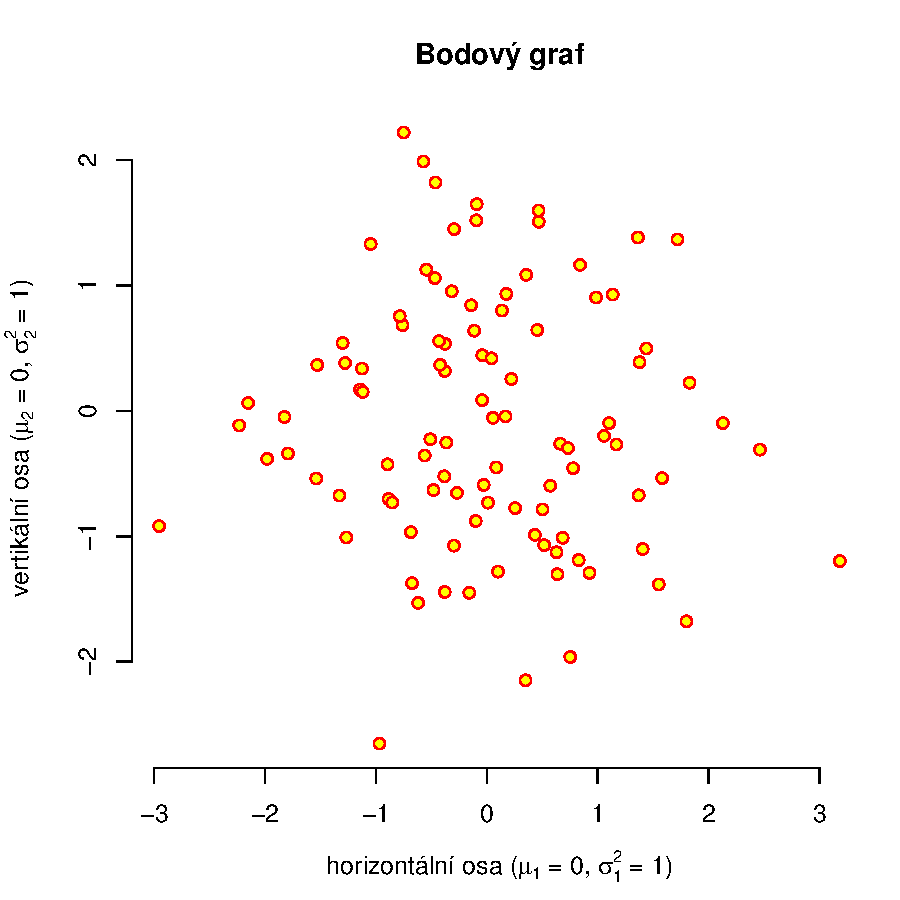
\includegraphics[width=140mm, height=140mm]{../img/ukazka-obr01}
% Příponu není potřeba explicitně uvádět, pdflatex automaticky hledá pdf.
% Rozměry také není nutné uvádět.
\caption{Náhodný výběr z~rozdělení $\mathcal{N}_2(\boldsymbol{0},\,I)$.}
\label{obr03:Nvyber}

\end{figure}

\begin{figure}[p]\centering
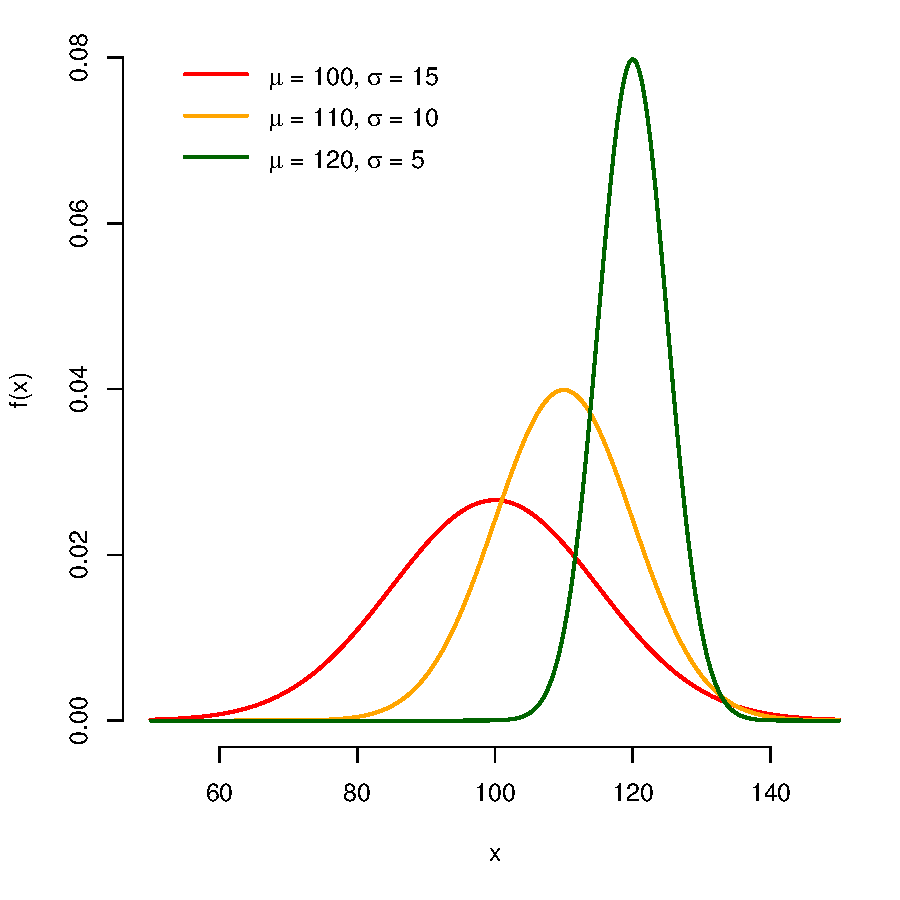
\includegraphics[width=140mm, height=140mm]{../img/ukazka-obr02}
\caption{Hustoty několika normálních rozdělení.}
\label{obr03:Nhust}
\end{figure}

\begin{figure}[p]\centering
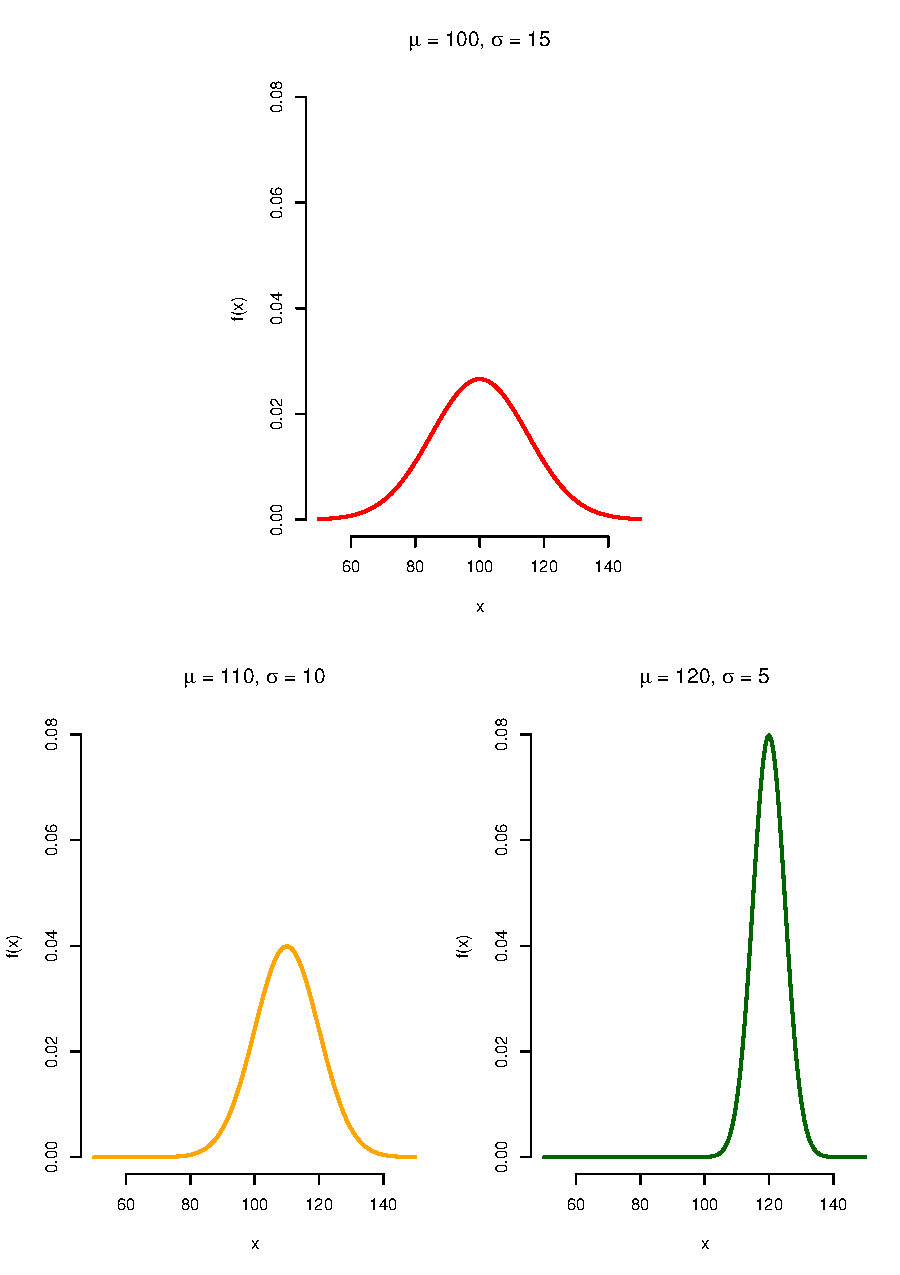
\includegraphics[width=140mm, height=198mm]{../img/ukazka-obr03}
\caption{Hustoty několika normálních rozdělení.}
\label{obr03:Nhust:podruhe}

\end{figure}
